%%%%%%%%%%%%%%%%%%%%
\chapter{Background}
% The background section introduces the necessary background to understand your work. This is not necessarily related work but technologies and dependencies that must be resolved to understand your design and implementation.
% This section is usually 3-5 pages.
%%%%%%%%%%%%%%%%%%%%

This chapter introduces the background material related to the NPP and the cybersecurity of its associated ICS.

\section{The Reactor Containment Building in a Nuclear Power Plant}

As the demonstrator attack targets a NPP equipment, this section briefly summarizes the plant operation and associated cyber and safety risks with a focus on the role of the targeted equipment — the polar crane. 

\subsection{Nuclear Power Plant (NPP)}

\emph{Nuclear Power Plants} (NPP) are using nuclear fission in order to heat water into steam which spins a turbine combined with a generator to produce electricity. In France, in 2023, all of the 56 civilian nuclear power reactors in operation, distributed in 16 nuclear power stations, are Pressurized Water Reactors. PWR are the most common type of nuclear reactor and as such are the ones considered in this project. A simplified view of a \emph{Pressurized Water Reactor} (PWR) can be found in~\autoref{fig:pwr}. As an electrical production site, NPP are considered as CI. Moreover, the NPP criticity is increased because of the nuclear fuel handling. The worst-case scenario to avoid is the radioactive contamination. It can for example happen in case of uncontrolled nuclear meltdown in the reactor vessel. 

Our cyberattack considers a particular situation of the NPP — its shutdown. The NPP shutdowns take place for maintenance, fuel reloading or ten-yearly inspection reasons.


\subsection{Reactor Containment Building (CB)}

The reactor \emph{Containment Building} (CB), or reactor building, is a containment structure in which we find the primary circuit and a part of the secondary circuit. A cross section of the CB can be found in~\autoref{fig:reactor_building}. The goal of this enclosure is to confine fission products. In return, large equipment cannot be easily delivered and must be delivered by the polar crane.

\subsection{Rotary Overhead Crane}

\begin{figure}[H]
    \centering
    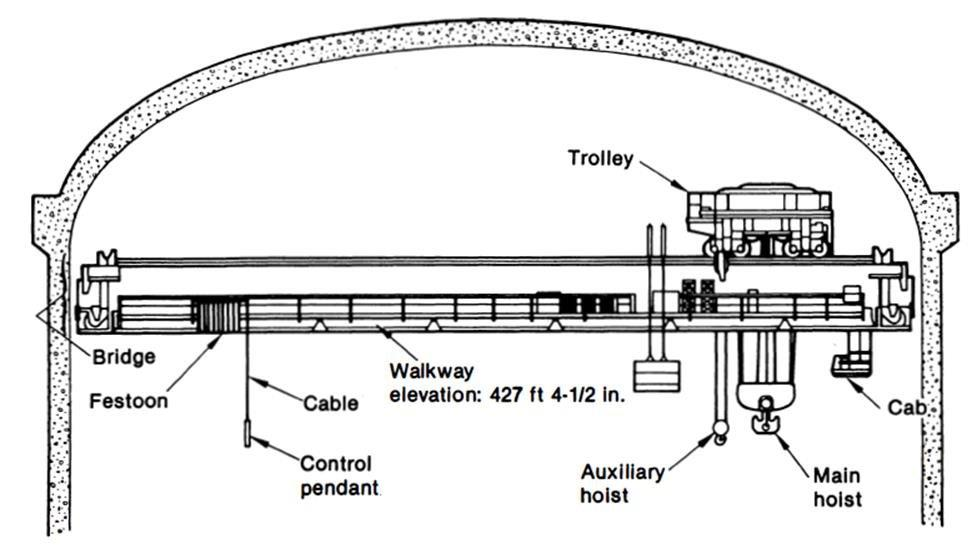
\includegraphics[height=8cm]{figures/rotary_crane.jpg}
    \caption{Rotary Overhead Crane~\cite{ONR-polar-crane}, or Polar Crane.  Three movements are possible in this system: polar crane rotation, trolley horizontal shift and charge lifting.}
    \label{fig:polar_crane}
\end{figure}

The attack demonstrator targets the polar crane's ICS. The operation of the polar crane is explained in this section. The rotary overhead crane (called thereafter polar crane) is a handling equipment which delivers and transports large components. It is for example used to lift and remove the reactor cover. The polar crane is only used during NPP shutdown, and its ICS is shutdown during the NPP operation. The polar crane equipment is standalone and is locally and manually operated by an operator. 

Two OT cyberattack scenarios were identified as possible ways of creating maximal damage and significant safety event:

\begin{itemize}
\item Shutdown of the polar crane with a charge above the reactor. This would create significant safety event with a possibility of the charge being drop above the reactor and breaking the first three barriers to radioactive release (i.e., fuel matrix, fuel cladding and boundary of the reactor coolant system)~\cite{international1996iaea}.
\item Activate charge lifting of the polar crane when it is in an overload situation caused by friction. For example this situation could be caused by friction when lifting a concrete slab which is placed above the confinement pool. If a cyberattacker detects it and  has full control over the PLC he could activate charge lifting to increase the overload which could either break the charge or make it fly.
\end{itemize}

\section{Industrial Control System and Programmable Logic Controller}

In this section are presented a cybersecurity introduction of the \emph{Industrial Control System} (ICS) and its major component — the \emph{Programmable Logic Controller} (PLC). 

\subsection{Industrial Control System (ICS)}

\emph{Industrial Control System} (ICS) is a network of interconnected systems that are designed to monitor and control industrial processes. Cybersecurity threats to ICS have far-reaching implications that can result in severe damage to property, loss of production, and even potential loss of life. Security of ICS thus requires a comprehensive approach that includes risk assessment, vulnerability identification, and implementation of appropriate protective measures.

ICS architecture are often modeled by the \emph{Purdue Model} represented in~\autoref{fig:purdue-model}. The attack surface is large and very diverse. It is large because the cyberattack could target any systems within the production network, the \emph{Industrial Control System} (ICS), the \emph{Supervisory Control And Data Acquisition} (SCADA), the corporate network etc. Attack surface is diverse because of the large number of different device types — actuators, sensors, \emph{Industrial Internet of Things} (IIoT) and smart devices, \emph{Remote Terminal Unit} (RTU), PLC, Engineering Workstation, \emph{Human-Machine Interface} (HMI), servers, switches, routers etc.


\subsection{Programmable Logic Controller (PLC)}

\emph{Programmable Logic Controller} (PLC), or similarly \emph{Programmable Automation Controller (PAC)}, is an industrial microprocessor-based controller made of a CPU, ROM, RAM, OS and a firmware. The PLC stacks are represented in~\autoref{fig:plc-stack}. The studied PLC is the \emph{Modicon M580} \emph{BMENOC0301} maintained by \emph{Schneider Electric}. It supports for example the following communication protocols: Modbus TCP, Ethernet IP, HTTP, FTP etc. The M580 is programmed by an engineering workstation by using the \emph{Unity Pro XL} software renamed as \emph{EcoStruxure Machine Expert} in the later versions. To program the PLC the closed-source Modbus/UMAS protocol is being used. 

\begin{figure}
    \centering
    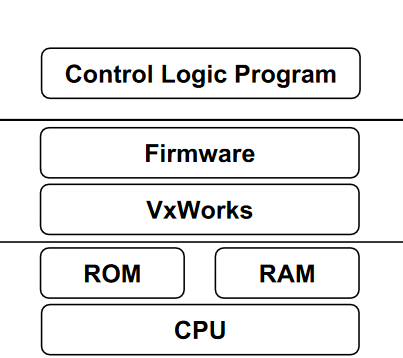
\includegraphics{figures/PLC-stacks}
    \caption{PLC Stacks of a PLC~\cite{Gao21} designed following the IEC 61131 standard. The Control Logic Program is the program executed by the CPU; it is a STM extension file for Schneider Electric programs. Considered firmware in this study is the Modicon M580 SV2.7 firmware. Considered CPU in this study is the Modicon M580. VxWorks is the real-time operating system running on the CPU.}
    \label{fig:plc-stack}
\end{figure}

\section{About Cybersecurity in ICS}

In the nuclear sector, most of the systems ensuring safety used to rely on analog devices. This technology adds a cybersecurity layer as analog devices are less complex and less connected. However, in the last decades, numerical devices with greater capabilities have penetrate the industrial market while the number of analog device manufacturers has dropped. This technology shift led to the success of several attacks~\cite{Drias15}. On another hand, the nuclear industry specifically focus on a defense-in-depth approach to ensure operational security.  

\subsection{Previous Major ICS Attacks in the Energy Sector}

\subsubsection{\emph{Stuxnet}}

\emph{Stuxnet} attack~\cite{stuxnetcode15},~\cite{Kushner13},~\cite{stuxnetdossier10} targeted the Iran's nuclear facilities and involved the use of a sophisticated worm exploiting multiple zero-day vulnerabilities and a rootkit technique to hide from antivirus. This OT cyberattack was designed to cause significant damage to the centrifuges responsible for enriching uranium by carefully tampering their speed to 1,064 cycles per second while keeping the attack stealth and persistent. The attackers used an attack cycle made of a combination of spear-phishing and network infiltration techniques to gain access to the targeted facility. Once inside, they deployed the \emph{Stuxnet} worm, which was capable of infecting both Windows operating systems and Siemens PLC while remaining undetected. 

\emph{Stuxnet} relied on several vulnerabilities to carry out its mission successfully. Primary vulnerability, the .LNK W32/\emph{Stuxnet} (CVE-2010-2568) vulnerability, took advantage of the use of USB drives to transfer data between systems. The associated exploit drops the trojan when the system automatically parses a shortcut file (.lnk)  which results in the execution of a malicious Control Panel module malware. This USB-based attack does not require to reprogram the USB peripheral. \emph{Stuxnet} approach allows replication by infecting USB thumb drives. \emph{NinjaCrane} is using another type of USB-based attack based on HID injection, which requires the presence of a programmable micro-controller in the USB peripheral. This adds a difficulty layer to the attacker and a less stealth attack but it allows in counter-part to infect any OS not implementing HID spoofing protection measures.

Another vulnerability that the attackers exploited was the weak authentication protocols of the \emph{Siemens} control systems. \emph{NinjaCrane} similarly exploits another vulnerability — \emph{ModiPwn} caused by a weak authentication of the \emph{Schneider Electric} communication protocol.

\subsubsection{\emph{Triton}}

The \emph{Triton} attack is a sophisticated cyberattack that targeted the safety instrumentation systems of a Saudi Arabian petrochemical plant in 2017. The \emph{Triton} attack started with the compromise of the plant’s network through phishing. The \emph{Triton} malware, once installed, was manipulating the safety controllers (the \emph{Triconex} PLC from \emph{Schneider Electric}) and the plant’s safety systems that monitor and detect incidents. By doing so, the attackers could have overridden the safety protocols, potentially resulting in an explosion or a toxic gas leak.

First vulnerability exploited was the human factor — the plant’s employees. The attackers used a spear-phishing email to trick an employee into downloading the \emph{Triton} malware, which then spread throughout the entire network. This highlights the importance of employees training in preventing cyberattacks.

One key vulnerability that the attackers exploited was the plant’s reliance on poorly-protected safety systems. The safety systems of the plant were not adequately secured against cyberattacks, and the use of legacy equipment, outdated firmware, and poorly configured network architecture made it easier for the attackers to breach the system and install the \emph{Triton} malware. The attackers were also successful in infiltrating the system because they had prior knowledge of the plant’s network topology, protocols, and industrial control systems, which helped them in crafting the malware to exploit the system’s vulnerabilities.

Similarities can be noted with the \emph{NinjaCrane} attack — the potentially catastrophic disaster of the cyberattack, human-factor role in the cyberattack, and prerequisite to reverse-engineer the PLC's communication protocol. This communication protocol is called \emph{TriStation} for the \emph{Triconex} PLC and Modbus/UMAS for the \emph{M580 PLC}. Also, the malware is, as for the \emph{NinjaCrane} attack, a python script compiled in an exe file using the \emph{py2exe} extension. Even if \emph{NinjaCrane} has persistence capabilities, it does not implement advanced hiding and anti-forensics techniques like \emph{Triton} does.

\subsection{From Operational Security to Cybersecurity in the Nuclear Industry}

The defense-in-depth approach taken by the nuclear industry during the control system design integrates operational security. The operational security can for example result into material and software redundancy, system qualification, human-supervision, mechanical stops, safety levels, priority on actuation control system etc. Those various mitigation barriers could also act as cybersecurity barriers. For example, a polar crane can integrate a kinematics line monitoring system responding to motor overspeed or engine backfire. As another example, a polar crane can integrate a wired emergency stop with highest priority order to shutdown the polar crane. Those defense-in-depth barriers won't protect directly against the \emph{NinjaCrane} attack but will prevent the attack to set a high polar crane's rotation speed or to deviate visually from normal operation as the automation operator will activate an emergency stop as soon as the the polar crane behaves differently than expected. 


\subsection{Security of the \emph{Modicon M580}}

\emph{Schneider Electric} lists all released vulnerabilities and their state \cite{schneider-portal-vuln}. As a first observation, the number of discovered vulnerabilities on the \emph{M580} is around ten per year. Moreover, the average time to patch a vulnerability is between two and four years. Unfortunately, patch deployment implies some code modification and thus requires a system re-qualification. It also requires industrial process stop. For those reasons a patch deployment can take more than a decade to be applied.

Among those vulnerabilities, the approach was to choose a communication protocol vulnerability as it allows to perform lateral movement from engineering workstation to PLC. Compromising directly the PLC would have require an access to the PLC. But the access to an ICS is physically restricted and PLC are usually placed into physically locked electrical cabinet. Moreover, in case of communication protocol vulnerability, remediation requires PLC firmware update and Unity Pro engineering workstation update. As date of 12 March 2023, Schneider Electric reports that a replay attack on the \emph{Modicon M580} is still possible \cite{schneider-replay-attack} and advises to harden the engineering workstation.

\subsection{Overview on USB-related Threats}

Number of USB-based attacks tends to increase over time and be more diverse~\cite{Nissim17}. \emph{NinjaCrane} makes use of a USB-based attack that can be classified as programmable micro-controller hardware-based attack. Many such attack-capable devices are available on the market, e.g., \emph{BadUSB}, \emph{BadUSB 2}, \emph{Rubber Ducky}, \emph{USBHarpoon}, \emph{OMG Cables}, \emph{USB Ninja}, \emph{Bash Bunny} etc.

\emph{NinjaCrane} infects the ICS with the use of a \emph{USB Ninja} cable type-C (or a maliciously modified mouse) that would be plugged to the engineering workstation. The USB Ninja cable and the malicious mouse are \emph{Human Interface Devices} (HID) spoofing device injecting keyboard key-frames. For the USB Ninja cable, the attack can be triggered over Bluetooth and in its professional version the key-frames can even been sent over Bluetooth. Moreover, the \emph{USB Ninja} cable is a working charging cable indistinguishable, at first glance, from a conventional charging cable. For the maliciously tampered mouse, any HID-capable device with extensive memory or embedded wireless connection can be placed in the mouse to execute the malware. Except from its weights, the mouse is indistinguishable from a conventional mouse.

\emph{Human Interface Device} (HID) spoofing device~\cite{epstem1225679} mimics legitimate HID to trick the computer to believe a keyboard is attached, the device then sends pre-configured keystrokes. To mimic a legitimate HID, the spoofing device operates an USB transport layer enumeration. It will then initiate data exchange under the format of input/output reports where the input report can contain keystrokes or mouse click to inject. As those keystrokes injection are impractical to deploy an advanced threat, the injected keystrokes generally perform an USB Drive-By attack in order to execute a downloaded malware.